\documentclass[11pt]{article}

\usepackage{sectsty}
\usepackage{graphicx}
\usepackage{enumitem}
\usepackage{listings}
\usepackage{xcolor}
\usepackage{graphicx}

\definecolor{codegreen}{rgb}{0,0.6,0}
\definecolor{codegray}{rgb}{0.5,0.5,0.5}
\definecolor{codepurple}{rgb}{0.58,0,0.82}
\definecolor{backcolour}{rgb}{0.95,0.95,0.92}

\lstdefinestyle{mystyle}{
    backgroundcolor=\color{backcolour},   
    commentstyle=\color{codegreen},
    keywordstyle=\color{magenta},
    numberstyle=\tiny\color{codegray},
    stringstyle=\color{codepurple},
    basicstyle=\ttfamily\footnotesize,
    breakatwhitespace=false,         
    breaklines=true,                 
    captionpos=b,                    
    keepspaces=true,                 
    numbers=left,                    
    numbersep=5pt,                  
    showspaces=false,                
    showstringspaces=false,
    showtabs=false,                  
    tabsize=2
}

\lstset{style=mystyle}


% Margins
\topmargin=-0.45in
\evensidemargin=0in
\oddsidemargin=0in
\textwidth=6.5in
\textheight=9.0in
\headsep=0.25in

\title{ 2021 Spring}
\author{ Web Technology Solution }
\date{\today}



\begin{document}
\maketitle	
\tableofcontents
\pagebreak

% Optional TOC
% \tableofcontents
% \pagebreak

%--Paper--

\section{(Q No.1 A) What is web hosting? Explain any 4 types of web hosting.}

\paragraph{}
Web hosting is a service that stores your website or web application and makes it easily accessible across different devices such as desktop, mobile, and tablets. Any web application or website is typically made of many files, such as images, videos, text, and code, that you need to store on special computers called servers. The web hosting service provider maintains, configures, and runs physical servers that you can rent for your files.

The four types of web hosting are:
\begin{enumerate}

    \item Shared hosting
        \subparagraph{}
        Shared hosting is a type of hosting service where the server resources like disk, memory, cpu are shared among others users using the same web server. Only the resources are shared among the users but not the website content, files, directory. 
        \subitem Advantages of shared hosting
        \begin{enumerate}
            \item Since the resources are shared among users, the cost of hosting will be cheap.
            \item Multiple websites can be hosted from single account
            \item Ease of setup and restart the services.
        \end{enumerate}

        \subitem Disadvantage of shared hosting
        \begin{enumerate}
            \item If one website get the high number of traffic then it will consume most of resources affecting other website performance.
            \item Limited access to configuraiton and installation of 3rd party software.
            \item Cost may increase substantialy as traffic increases
        \end{enumerate}

    \item VPS hosting
    \subparagraph{}
    Virtual private server (VPS) hosting providers use a virtual private server to give more exclusive access to server resources. VPS hosting technology partitions the physical server to create small virtual servers that for lease. With virtual private servers, we can have exclusive access to both space and computing resources, such as memory and processing power, on the physical server. We can install an operating system on your virtual server and have greater control of your server environment.
    It is very suitable for: 
    \begin{enumerate}
        \item medium sized business with high traffic
        \item websites requires other software installation
    \end{enumerate}
    \subitem Advantages of VPS hosting
    \begin{enumerate}
        \item Provides complete controle over the server.
        \item Greater control over website performance
    \end{enumerate}
    \subitem Disavantages of VPS hosting
    \begin{enumerate}
        \item Requires inhouse technical experts to maintaing the servers.
    \end{enumerate}

    \item Dedicated hosting
    \subparagraph{}
    Dedicated hosting give access to the complete physical server with exclusive access to a dedicated server. We can optimize and control the environment as per requirements. We can partition this server to host multiple domains on the same physical server.
    This is suitable for:
    \begin{enumerate}
        \item large enterprises and business
        \item business owners with multiple services
        \item Web application with heavy processing powers required
    \end{enumerate}
    \subitem Advantages of Dedicated hosting
    \begin{enumerate}
        \item Very reliable and secured
        \item Access to server optimization capablitlies
        \item Customization of server conf
    \end{enumerate}
    \subitem Disadvantages of Dedicated hosting
    \begin{enumerate}
        \item Very expensive to lease and maintain
        \item Required inhouse technical experts
    \end{enumerate}

    \item Cloud hosting
    Cloud hosting is a hosting service which uses resource sharing and scale to decrease web hosting costs and improve website performance. We can get shared access to a cluster of servers, and the cloud hosting provider automatically replicates website files across several servers. If one of the cloud servers is busy, the hosting provider automatically routes your traffic to another server. This greatly improves website performance without adding to your ongoing costs. 
    This is suitable for:
    \begin{enumerate}
        \item small and medium business
        \item Complex web application with multiple services
        \item Large enterprises with several domain
    \end{enumerate}
    \subitem Advantages of Cloud hosting
    \begin{enumerate}
        \item Greater availability and reliability for your website users.
        \item Automatically scales up or down as your requirements change.
        \item High flexibility—you pay for only what you use.
    \end{enumerate}
    \subitem Disadvantages of Cloud hosting
    \begin{enumerate}
        \item Vulnerable to attack
        \item Requires technical expert to maintain the servers requirement
    \end{enumerate}
\end{enumerate}


\pagebreak
\section{(Q No.1 B) What is mime type specification in request/response transaction between browser and server?}
\subparagraph{}
In a request/response transaction between a browser and server, the MIME type specification is used to indicate the type of data that is being transmitted in the HTTP message. The MIME (Multipurpose Internet Mail Extensions) type is a standardized way to specify the format of data in Internet messages, and it helps the browser to know how to handle the content it receives from the server.

When a browser sends a request to a server, it includes an Accept header in the request message, which lists the MIME types that the browser can handle. The server then sends the response back to the browser, along with a Content-Type header that specifies the MIME type of the data being sent.

For example, if a user requests a webpage that contains an image, the browser will send a request to the server asking for the image file. The server will respond with the image data and a Content-Type header that specifies the MIME type of the image, such as "image/png" for a PNG file.

Similarly, when a user submits a form with data, the browser will send a request to the server with a Content-Type header that specifies the MIME type of the data being sent, such as "application/x-www-form-urlencoded" or "multipart/form-data".

By using MIME type specification, browsers and servers can communicate effectively and ensure that the data being transferred is interpreted correctly.

A MIME type is a string identifier composed of two parts: a type and a subtype.
\begin{enumerate}
    \item "type" refers to a logical grouping of many MIME types that are closely related to each other; it's no more than a high level category.
    \item "subtypes" are specific to one file type within the "type".
\end{enumerate}

\subparagraph{Examples of MIME types are:}
\begin{enumerate}
    \item text/html for normal web pages
    \item text/plain for plain text
    \item application/octet-stream meaning “download this file”
    \item application/x-java-applet for Java™ applets
    \item application/pdf for Adobe® PDF documents.
\end{enumerate}

\pagebreak

\section{(Q No. 2A) What are the different typs of list available in HTML? Explain each with suitable availabe code.}
\subparagraph{}
There are 3 types of list in HTML:

\subparagraph{Unordered List or Bulleted List (ul)} 
    This list is used when there is no specific order or sequence. An unordered list is also called a Bulleted list, as the items are marked with bullets. It begins with the 〈ul〉 tag and and closes with a 〈/ul〉 tag. The list items begin with the 〈li〉 tag and end with 〈/li〉 tag.
    \begin{lstlisting}[language=html, caption=Unordered list example]
        <ul>
        <li>Apple</li>
        <li>Mango</li>
        <li>Banana</li>
        <li>Grapes</li>
        <li>Orange</li>
     </ul>
    \end{lstlisting}
\subparagraph{Ordered List or Numbered List (ol)}
The list items in an ordered list are marked with numbers by default instead of bullets. An HTML ordered list starts with the 〈ol〉 tag and ends with the 〈/ol〉 tag. The list items start with the 〈li〉 tag and end with 〈/li〉 tag.
    \begin{lstlisting}[language=html, caption=Ordered list example]
        <ol>
        <li>Apple</li>
        <li>Mango</li>
        <li>Banana</li>
        <li>Grapes</li>
        <li>Orange</li>
     </ol>
    \end{lstlisting}
\subparagraph{Description List or Definition List (dl)}
the list items are listed like a dictionary or encyclopedia. Each item in the description list has a description. You can use a description list to display items like a glossary. You will need the following HTML tags to create a description list:
\begin{enumerate}
    \item 〈dl〉 (Definition list) tag - Start tag of the definition list
    \item 〈dt〉 (Definition Term) tag - It specifies a term (name)
    \item 〈dd〉 tag (Definition Description) - Specifies the term definition
    \item 〈/dl〉 tag (Definition list) - Closing tag of the definition list

\end{enumerate}
\begin{lstlisting}[language=html, caption=Description list example]
    <dl>
    <dt><b>Apple</b></dt>
    <dd>A red colored fruit</dd>
    <dt><b>Honda</b></dt>
    <dd>A brand of a car</dd>
    <dt><b>Spinach</b></dt>
    <dd>A green leafy vegetable</dd>
 </dl>
\end{lstlisting}


\section{(Q No. 2B) Write Html tags to generate following form.}
% TODO: include image of form
\lstinputlisting[language=html]{resources/qno2b.html}


\section{(Q No. 3A) What are the different level of stylesheets with their hierarchy of implementation? Explain the float and clear properties with clear and valid example?}
\subparagraph{}
There are 3 levels of stylesheets in CSS:
\begin{enumerate}
    \item Inline Styles: These styles are applied directly to an HTML element using the style attribute. Inline styles have the highest specificity, meaning they override any other styles applied to the same element.
    \begin{lstlisting}[language=html, caption=Inline Style]
        <p style="color: red;">This text is red.</p>
    \end{lstlisting} 

    \item Internal Styles: These styles are defined within the head section of an HTML document using the style tag. Internal styles have a higher specificity than external styles, but lower than inline styles.
    \begin{lstlisting}[language=html, caption=Internal Style]

        <head>
    <style>
        p {
        color: blue;
        }
    </style>
    </head>
    <body>
    <p>This text is blue.</p>
    </body>
    \end{lstlisting} 
    
    \item External Styles: These styles are defined in an external CSS file and are linked to an HTML document using the link tag. External styles have the lowest specificity, but they are also the most reusable and easier to maintain.
    \begin{lstlisting}[language=html, caption=External Style]
    
    <head>
  <link rel="stylesheet" href="style.css">
</head>
<body>
  <p class="red-text">This text is red.</p>
</body>
\end{lstlisting} 

\subparagraph{}
Float is a CSS property used to move an element to the left or right of its container, allowing other elements to flow around it. 
The clear property is used to force an element to be placed below any floated elements.
\begin{lstlisting}[language=html, caption=Internal Style]
<style>
  .box {
    width: 200px;
    height: 200px;
    float: left;
    margin-right: 10px;
  }
  .clear {
    clear: both;
  }
</style>

<div class="box" style="background-color: red;">red</div>
<div class="box" style="background-color: blue;">blue</div>
<div class="clear"></div>
<div class="box" style="background-color: green;">green</div>
\end{lstlisting} 
Here in the example above, we have three boxes floated to the left. The second box is positioned next to the first box because of the float property. However, we want the third box to be placed below the floated boxes, so we add a div with the clear property to force it to the next line.

% clear_float.PNG
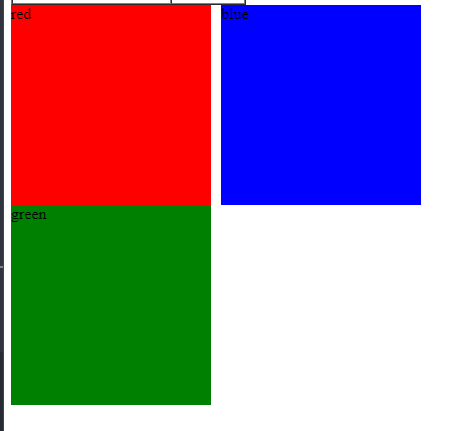
\includegraphics{./resources/clear_float.PNG}

\end{enumerate}

\section{(Q No. 3B) What are the logical and physical tags? Give examples also.}
\subparagraph{}
In Html there are 2 types of tags: 
\begin{enumerate}
    \item Logical tags are used to describe the purpose or meaning of the content. They are used to tell the browser to tell what kind of text is written inside the tags. 
    Logical tags are also called Structural tags.
    Logical tags are used to indicate to the visually impaired person that there is something more important in the text or to emphasize the text ie, logical tags can be used for styling purposes as well as to give special importance to text content.

    Here are some examples of logical tags:
\begin{lstlisting}[language=html, caption=logical tags]
    <h1>, <h2>, <h3>, <p>, <ul>, <ol>, <li>, <table>, <form>, etc.
\end{lstlisting} 

Here are the usecases of logical tags
    \begin{enumerate}
        \item To write code on our website.
        \item To Emphasize some text.
        \item To display the abbreviation on the Web page.
        \item To display some famous quotation on our web page.
        \item To write some mathematical formula in terms of variables.
    \end{enumerate}
    
    Logical tags are used to structure the content of a web page and give it semantic meaning. For example, the \textlangle h1 \textrangle tag is used to indicate the main heading of a page, while the \textlangle p \textrangle tag is used to define a paragraph of text.
    
    \item Physical tags:
    Physical tags are used to indicate that how specific characters are to be formatted or indicated using HTML tags. Any physical style tag may contain any item allowed in text, including conventional text, images, line breaks, etc. Physical tags can only be used for styling purposes for specific elements. Although each physical tag has a defined style, you can override that style by defining your own look for each tag. All physical tags require ending tags
    Here are the few physical tags.
    \begin{lstlisting}[language=html, caption=physical tags]
    <b>, <i>, <u>, <strike>, <font>, <center>, <br>, <hr>, etc.
    \end{lstlisting} 
    Here are the usecases of Physical tags:
    \begin{enumerate}
        \item  They are extremely straightforward.
        \item  They are used to highlighting important sentences.
        \item  Physical Text Styles indicate the specific type of appearance for a section e.g., bold, italics, etc.
        \item  Physical Styles are rendered in the same manner by all browsers.
    \end{enumerate}
    Physical tags are used to define the appearance of the content on a web page. For example, the \textlangle b \textrangle tag is used to make text bold, while the \textlangle i \textrangle  tag is used to make text italic. The \textlangle br \textrangle tag is used to insert a line break, while the \textlangle hr \textrangle tag is used to insert a horizontal line.

\end{enumerate}


\section{(Q No. 3C) What do you mean by table-less design and how will you achieve it using CSS?}
\subparagraph{}
    Table-less design, also known as CSS-based design, is an approach to web design that avoids using HTML tables for layout purposes. Instead, it uses CSS (Cascading Style Sheets) to control the layout and presentation of the content on a web page.

    The primary advantage of table-less design is that it allows for more flexible and accessible web design, as well as faster load times. It also separates the content and presentation of a web page, making it easier to update and maintain.
    
    To achieve table-less design using CSS, here are some key steps:
    
        \begin{enumerate}
            \item Using semantic HTML: Using logical tags such as 
            \begin{lstlisting}[language=html]
                <header>, <main>, <nav>, <section>, and <article>
            \end{lstlisting} 
            to structure the content of your web page, helps to separate the content and structure from the presentation.
    
            \item Using CSS layout techniques: Using CSS layout techniques such as Flexbox and CSS Grid to control the layout of the content on the web page. These techniques allow for more flexibility and control over the positioning of elements on the page.
    
            \item Use CSS for styling: Use CSS to control the presentation of the content on your web page. This includes setting fonts, colors, borders, and other visual properties.
    
            \item Avoid using HTML tables for layout: Use tables only for tabular data, not for layout purposes. Instead, use CSS layout techniques to achieve the desired layout.
    
            \item Test for accessibility: Test your web page for accessibility using tools such as screen readers and keyboard navigation. Ensure that the content is accessible to all users, including those with disabilities.
        \end{enumerate}
        \lstinputlisting[language=html]{resources/table-less.html}




\section{(Q No. 4A) What do you mean my DOM in javascript? How do you get elements from document to javascript? Write example of all methods.}
\subparagraph{}
The Document Object Model (DOM) is a programming interface for web documents. It represents the page so that programs can change the document structure, style, and content. With the DOM, JavaScript can access and manipulate the elements of an HTML or XML document.

Here are the methods to get elements from the document to JavaScript:
\begin{enumerate}
    \item  \textbf{document.getElementById():} This method returns the element with the specified ID. For example, to get the element with ID "myElement", we can get using the code
    \begin{lstlisting}[language=html]
        var myElement = document.getElementById("myElement");
    \end{lstlisting}

    \item  \textbf{document.getElementsByClassName():} This method returns a collection of elements with the specified class name. This method returns a collection, so we need to loop through the collection to access each element.
     For example, to get all elements with class name "myClass", we can use the following code:

    \begin{lstlisting}[language=html]
        var myElements = document.getElementsByClassName("myClass");
    \end{lstlisting}

    \item  \textbf{document.getElementsByTagName():} This method returns a collection of elements with the specified tag name. This method also returns a collection.
    For example, to get all p elements on the page, we can use the following code:

    \begin{lstlisting}[language=html]
        var myElements = document.getElementsByTagName("p");
    \end{lstlisting}

    \item  \textbf{document.querySelector():} This method returns the first element that matches a specified CSS selector. This method only returns the first matching element.
    For example, to get the first p element on the page, we can use the following code:

    \begin{lstlisting}[language=html]
        var myElement = document.querySelector("p");
    \end{lstlisting}

    \item  \textbf{document.querySelectorAll():} This method returns a collection of elements that match a specified CSS selector. This method also returns a collection.
    For example, to get all p elements with class "myClass", we can use the following code:

    \begin{lstlisting}[language=html]
        var myElements = document.querySelectorAll("p.myClass");

    \end{lstlisting}

With these methods, we can easily get elements from the document into JavaScript and manipulate them as needed.

\end{enumerate}


\section{(Q No. 4B) Write JavaScript program which validates the user data(name, email, contact no) and displays the success message if validated successfully. Also create HTML form for entering data.}
\lstinputlisting[language=java]{resources/qno4b.html}



\section{(Q No. 5A) What do you mean by events and events handling? Write HTML and JS code to display digital clock.}
\lstinputlisting[language=java]{resources/qno5a.html}


\section{(Q No. 5B) What are the different file handling methods available in PHP? After validating form value in 5(A) write the contents to the users.txt with time of login. Also redirect home.php after writing contents to the file. The content of file should look like this. 
Name: abs Sharma, Email: testuser@gmail.com Logged in on: Fri Feb 01 2020 17:00:00 GMT +0545 (Nepal Time)}
\subparagraph{}
PHP provides various file handling methods to read, write, and manipulate files. Here are some of the most commonly used file handling methods in PHP:
    \begin{enumerate}
        \item \textbf{fopen():} This function is used to open a file in PHP. It returns a file pointer, which is used by other file handling functions to perform operations on the file.

        \item \textbf{fclose():} This function is used to close a file that has been opened using fopen().
    
        \item \textbf{fread():} This function is used to read data from a file. It takes two parameters: the file pointer returned by fopen(), and the number of bytes to read.
    
        \item \textbf{fwrite():} This function is used to write data to a file. It takes two parameters: the file pointer returned by fopen(), and the data to write.
    
        \item \textbf{feof():} This function is used to check if the end of the file has been reached.
    
        \item \textbf{fgets():} This function is used to read a line from a file. It takes the file pointer returned by fopen() as a parameter.
    \end{enumerate}

    Here is the PHP code to achieve what is requested writing form data to file, with timestamp.
    \lstinputlisting[language=java]{resources/qno5b.php}


\section{(Q No. 6A) Explain the use of PHP \$\_POST, \$\_GET and \$\_REQUEST variables.}
\subparagraph{}
    In PHP, \$\_POST, \$\_GET, and \$\_REQUEST are superglobal variables used to collect data submitted in HTML forms, as well as data appended to the URL. Here's an explanation of each variable:

  \begin{enumerate}
    \item   \textbf{\$\_POST:} This variable is used to collect data that is submitted through an HTML form with the HTTP POST method. The data is encoded in the message body of the HTTP request. The data is accessible using the name attribute of the input field in the form. For example:
    \begin{lstlisting}[language=html, caption={form.html}]
        <form method="post" action="process.php">
        <label for="username">Username:</label>
        <input type="text" id="username" name="username">
        <label for="password">Password:</label>
        <input type="password" id="password" name="password">
        <button type="submit">Submit</button>
        </form>
    \end{lstlisting}
    In the example above, the \$\_POST variable can be used in process.php to get the values of the username and password fields:
    \begin{lstlisting}[language=php, caption={process.php}]
        $username = $_POST['username'];
        $password = $_POST['password'];
    \end{lstlisting}

    \item \textbf{\$\_GET:} This variable is used to collect data that is appended to the URL with the HTTP GET method. The data is visible in the URL query string, and can be accessed using the key-value pairs in the query string. For example:
    \begin{lstlisting}[language=html, caption={link.html}]
        <a href="profile.php?username=johndoe">View profile</a>
    \end{lstlisting}
    In the example above, the \$\_GET variable can be used in profile.php to get the value of the username parameter:
    \begin{lstlisting}[language=html, caption={profile.php}]
        $username = $_GET['username'];
    \end{lstlisting}

    \item \textbf{\$\_REQUEST:} This variable is used to collect data submitted through either \$\_POST or \$\_GET. The data can be accessed using the name attribute of the input field in the form or the key-value pairs in the query string. For example:
    \begin{lstlisting}[language=php, caption={process.php}]
        $username = $_REQUEST['username'];
    \end{lstlisting}

    In the example above, the \$\_REQUEST variable can be used to get the value of the username parameter regardless of whether it was submitted through \$\_POST or \$\_GET.

  \end{enumerate}

\section{(Q No. 5B) Write PHP-MySQL code validate the user login data (email and password). That is check whether the user data is available in database or not. Also in another file write code to display the user information (name and email). (Assume database name to "testdb" and table name is "users")}
\subparagraph{}
We first connect to the MySQL database using \[ mysqli\_connect\left(\right) \] function. We then check if the form has been submitted using \[ \$\_SESSION\left[ "REQUEST\_METHOD" \right] \] variable. If it has, we get the values of email and password fields using \$\_POST variable.

We then validate the user login data against the database by querying the users table using \[ mysqli\_query\left(\right) \] function. If the query returns a row, we start a session and set the email value to \[ \$\_SESSION\left[ "email" \right] \]. We then redirect to userinfo.php using \[header()\] function. If the query returns no rows, we display an error message.
Here is the login.php file source code for logging in users.
\lstinputlisting[language=php, caption={login.php}]{resources/login.php}

We then check if the user is logged in by checking if \[ \$\_SESSION\left[ "email" \right] \]  is set. If it is not set, we redirect to login.php using header function.

If the user is logged in, we get the user information from the database by querying the users table using \[ mysqli\_query\left(\right) \] function. If the query returns a row, we display the user information. If the query returns no rows, we display an error message

Here's an example PHP-MySQL code to display user information based on the email value stored in the session:
\lstinputlisting[language=php, caption={userinfo.php}]{resources/users.php}

\section{(Q No. 7A) Hyperlinks and Hypermedia}
\subparagraph{}
Hyperlinks and hypermedia are concepts related to linking and navigating between web pages and resources.

Hyperlinks are links that allow users to navigate from one web page to another by clicking on them. Hyperlinks can be represented as text, images, or other types of media and are usually highlighted or underlined to indicate that they are clickable. For example, clicking on a hyperlink in a blog post may take you to a related article or another website.

Hypermedia, on the other hand, refers to the use of different types of media, such as text, images, video, and audio, to link and navigate between resources. In addition to linking to other web pages, hypermedia can also link to different types of media files, such as images or videos. For example, a hypermedia document may contain clickable images that take users to related articles or videos.

Hyperlinks and hypermedia are fundamental concepts in web design and are used to create intuitive and interactive user experiences. They allow users to navigate between related content and resources, helping them to discover and consume information more easily.
Here are some example of hyperlink and hypermedia
\begin{enumerate}
    \item \textbf{Hyperlink} This creates hyperlink to a website.
    \[ <a href="https://www.example.com">Click here to visit Example website</a>
\] 
    \item \textbf{Image Hyperlink} This code creates a clickable image that takes users to the website "https://www.example.com" when clicked. The image file "example.png" is displayed as the clickable element.
    \[ <a href="https://www.example.com"><img src="example.png" alt="Example website"></a>
\]
    \item \textbf{Video Hyperlink} This code creates a hyperlink that links to a video file "video.mp4" located at "https://www.example.com". When clicked, the video will start playing.
     \[ <a href="https://www.example.com/video.mp4">Watch the video here</a>
\]
    \item \textbf{Hypermedia} This code creates a clickable element that includes an image and text. When clicked, users will be taken to the website "https://www.example.com". The image and text provide additional context and information about where the hyperlink will take them.
    \[ <a href="https://www.example.com">
    <img src="example.png" alt="Example website">
    <p>Click here to visit Example website</p>
  </a>
\]  
\end{enumerate}
\section{(Q No. 7B) Pop up boxes in JavaScript}
\subparagraph{}
Pop up boxes in JavaScript are used to display messages or alerts to users. There are three types of pop up boxes in JavaScript: alert boxes, confirm boxes, and prompt boxes.

\begin{enumerate}
    \item \textbf{Alert Boxes} Alert boxes are used to display a message to the user. They are useful for displaying important information that requires the user's attention. Here's an example:
    \begin{lstlisting}
        alert("Hello, World!");   
    \end{lstlisting}
    \item \textbf{Confirm Boxes:}
    Confirm boxes are used to ask the user to confirm or cancel an action. They are useful for getting the user's input before performing an action that could have consequences. Here's an example:
    \begin{lstlisting}[language=python]
        if (confirm("Are you sure you want to delete this item?")) {
        // Perform the deletion
      } else {
        // Cancel the deletion
      }
    \end{lstlisting}
    When this code is executed, a confirm box will pop up with the message "Are you sure you want to delete this item?". If the user clicks the "OK" button, the code inside the if statement will be executed. If the user clicks the "Cancel" button, the code inside the else statement will be executed.
    \item \textbf{Prompt Boxes:}
    Prompt boxes are used to ask the user to enter some text. They are useful for getting input from the user before performing an action. Here's an example:
    \begin{lstlisting}
        var name = prompt("Please enter your name:");
        alert("Hello, " + name + "!");
    \end{lstlisting}
    When this code is executed, a prompt box will pop up with the message "Please enter your name:". The user can enter their name and click the "OK" button. The code then uses the entered name to display a personalized message.
\end{enumerate}


\section{(Q No. 7C) Types of array in PHP}
\subparagraph{}
In PHP, there are three types of arrays:
\begin{enumerate}
    \item \textbf{Indexed arrays:}
    An indexed array stores a collection of values, each of which is assigned a numeric index. The index starts at 0 and increases by 1 for each element in the array. Indexed arrays can be created using the array() function or using the shorthand [] syntax. Here's an example:
    \begin{lstlisting}[language=php]
        $fruits = array("apple", "banana", "orange");
        // or
        $fruits = ["apple", "banana", "orange"];
    \end{lstlisting}

    \item \textbf{Associative arrays:}
    An associative array stores a collection of key-value pairs, where each key is a string and each value can be of any type. Associative arrays can be created using the \[array()\] function or using the shorthand [] syntax, but the key-value pairs must be explicitly defined using the => operator. Here's an example:
    \begin{lstlisting}[language=php]
        $person = array("name" => "John", "age" => 30, "email" => "john@example.com");
        // or
        $person = ["name" => "John", "age" => 30, "email" => "john@example.com"];

    \end{lstlisting}

    \item \textbf{Multi dimensional array:}
    Multidimensional array is an array that contains one or more arrays as its elements. Each element of a multidimensional array can be an array itself, which can contain further arrays as its elements.

    Multidimensional arrays are useful for representing complex data structures, such as tables or matrices. They can be indexed using multiple sets of keys, which allows for flexible and efficient data access.
    \begin{lstlisting}[language=php]
        \$data = array(
            array("John", "Doe", 25),
            array("Jane", "Smith", 30),
            array("Bob", "Johnson", 40)
        );
    \end{lstlisting}
\end{enumerate}

%--/Paper--

\end{document}